\documentclass{amsart}

\usepackage[english]{babel}
\usepackage[utf8]{inputenc}
\usepackage{graphicx}
\usepackage{mathtools}
\usepackage{amsthm}
\usepackage{amsfonts}
\usepackage{hyperref}
\usepackage[singlelinecheck=false]{caption}
\usepackage{enumitem}
\usepackage[justification=centering]{caption}
\usepackage{indentfirst}
\usepackage{algorithm}
\usepackage{algpseudocode}
\usepackage{listings}

\makeatletter
\def\subsection{\@startsection{subsection}{3}%
  \z@{.5\linespacing\@plus.7\linespacing}{.1\linespacing}%
  {\normalfont\itshape}}
\makeatother

\DeclareMathOperator*{\argmin}{arg\,min}
\DeclareMathOperator*{\argmax}{arg\,max}

\newcommand\defeq{\mathrel{\overset{\makebox[0pt]{\mbox{\normalfont\tiny\sffamily def}}}{=}}}

\algrenewcommand\algorithmicrequire{\textbf{Input}}
\algrenewcommand\algorithmicensure{\textbf{Output}}

\captionsetup[table]{labelsep=space}

\theoremstyle{plain}

\newtheorem*{definition}{Definition}
\newtheorem{theorem}{Theorem}
\newtheorem{proposition}{Proposition}
\newtheorem{exercise}{Exercise}

\newcommand{\set}[1]{\mathcal{#1}}
\newcommand{\pr}{\mathbb{P}}
\renewcommand{\implies}{\Rightarrow}

\setlength{\parskip}{1em}

\title[]{EP1 -- MAC0438 -- Programação Concorrente}
\author[]{Renato Lui Geh\\NUSP\@: 8536030}

\begin{document}

\begin{abstract}
  Soluções dos exercícios bônus do Exercício Programa 1 de MAC0438 Programação Concorrente.
  \vspace*{-2.5em}
\end{abstract}

\maketitle

\section{Programa 1}

São criados quatro processos. Considere o seguinte grafo:

\begin{figure}[h]
  \centering{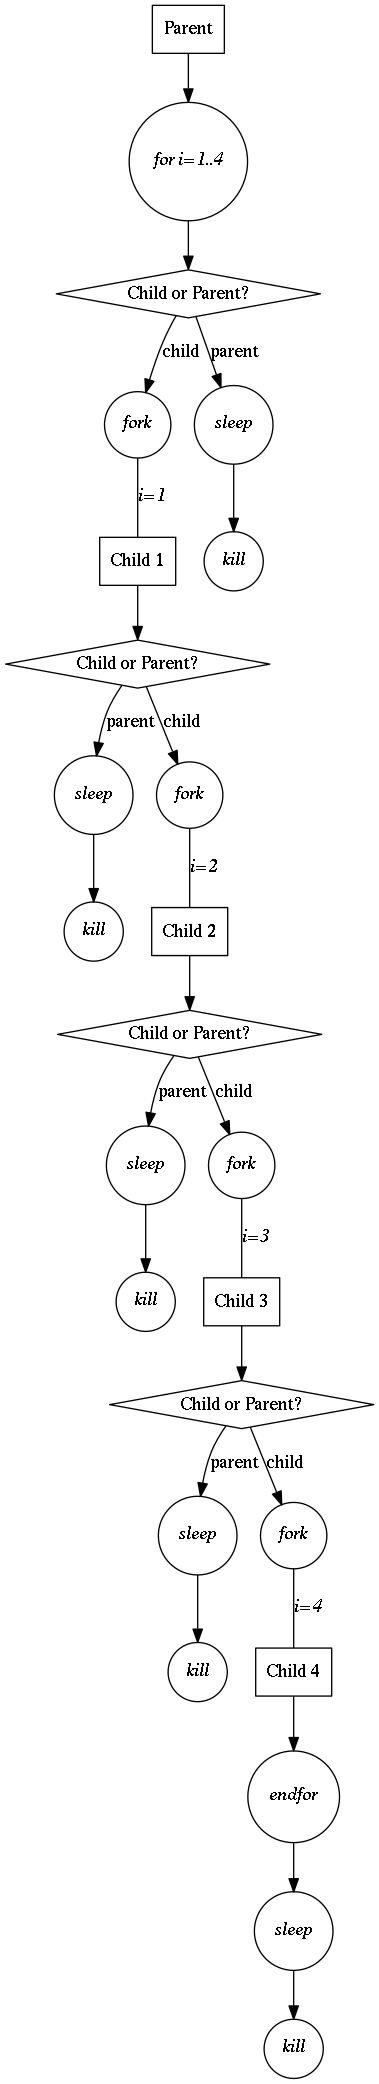
\includegraphics[scale=0.3]{graphs/p1.png}}
\end{figure}

É possível ver que, assim que cria-se um processo com \lstinline{fork}, o processo pai termina sua
execução. Os processos filhos tem sua paternidade automaticamente movida para o processo
\lstinline{init} pelo sistema operacional, o que guarante que os processos continuem rodando. Assim
que cada um acabar sua execução, a memória de cada processo é liberada.

\end{document}
